% !TeX program = lualatex
\documentclass[a5paper,11pt,openany]{article}
\usepackage{orcidlink}

\usepackage{blindtext}
%\usepackage[style]{abstract}

\usepackage[top=2cm,bottom=2cm,bindingoffset=0cm]{geometry}

\usepackage[svgnames]{xcolor} % Required to specify font color

%\documentclass[a4paper,12pt,openany]{scrbook}

%\usepackage{glossaries}
%\usepackage[xindy]{glossaries}
%\makeglossaries

%\usepackage{odsfile,lmodern}

%\usepackage{luacode}


\usepackage{multicol}

%\usepackage{churchslavonic}
%\usepackage{polyglossia}
%\setotherlanguages{russian,churchslavonic}

\usepackage{mathtext}
\usepackage{makeidx}
%\usepackage{imakeidx}
\usepackage{longtable}
\usepackage[tc]{titlepic}

\usepackage{fontspec}

\usepackage[protrusion=true,expansion,
tracking=true,letterspace=50]{microtype}


%\usepackage{academicons}
%\usepackage{xcolor}


%\SetTracking[ spacing = {25*,166, } ]{ encoding = *, shape = sc }{ 25 }


%\usepackage{soulutf8}
%\usepackage{letterspace}

%\usepackage[toc]{appendix}
\usepackage[toc,titletoc]{appendix}
\renewcommand\appendixtocname{Приложения}
\renewcommand\appendixpagename{Приложения}

%\usepackage{xunicode}
\usepackage{xltxtra}

\usepackage[normalem]{ulem}
\usepackage{adjustbox}

\usepackage{polyglossia}
\setmainlanguage{russian}
\setdefaultlanguage{russian}
\setotherlanguage{ukrainian}
\setotherlanguage{english}
\setotherlanguage{greek}
\setotherlanguage{latin}
\setotherlanguage{polish}


\setmainfont[BoldFont={DejaVuSerif-Bold.ttf},
ItalicFont={DejaVuSerif-Italic.ttf},
 BoldItalicFont={DejaVuSerif-BoldItalic.ttf}]{DejaVuSerif.ttf}

\setromanfont[BoldFont={DejaVuSerif-Bold.ttf},
ItalicFont={DejaVuSerif-Italic.ttf},
 BoldItalicFont={DejaVuSerif-BoldItalic.ttf}]{DejaVuSerif.ttf}

\setsansfont[BoldFont={DejaVuSans-Bold.ttf},
ItalicFont={DejaVuSans-Oblique.ttf},
 BoldItalicFont={DejaVuSans-Oblique.ttf}]
{DejaVuSans.ttf}

\setmonofont[BoldFont={DejaVuSansMono-Bold.ttf},
ItalicFont={DejaVuSansMono-Oblique.ttf},
 BoldItalicFont={DejaVuSansMono-BoldOblique.ttf}]
{DejaVuSansMono.ttf}



\usepackage{enumitem}
\usepackage{indentfirst} 

\usepackage{verse}

\usepackage{graphicx}

%\usepackage[pdfpagelabels,unicode,plainpages=false]{hyperref}

\hypersetup{pdftitle=Скотий бог Волос. Петр Семилетов.}

\usepackage{bookmark} 
\usepackage{relsize}

\usepackage{tocloft,calc}
\usepackage[nottoc,numbib]{tocbibind}


\frenchspacing
\righthyphenmin=2


\makeatletter
\@addtoreset{chapter}{part}
\makeatother  


%\titlepic{\includegraphics[width=0.50\textwidth]{cover/04.jpg}}

\title{CКОТИЙ БОГ ВОЛОС\\
\textsmaller[2]{редакция 1.0}}
\author{Петр Семилетов\\ORCID:0009-0002-3901-7785 \orcidlink{0009-0002-3901-7785}}
\date{24/11/2024}



\newcommand*{\plogo}{\fbox{$\mathcal{PL}$}} % Generic publisher logo

% –  –  –  –  –  –  –  –  –  –  –  –  –  –  –  –  –  –  –  –  –  –  –  –  –  –  –  –  –  –  –  –  –  –  –  –  –  –  –  –  –  –  –  – 
%	TITLE PAGE
% –  –  –  –  –  –  –  –  –  –  –  –  –  –  –  –  –  –  –  –  –  –  –  –  –  –  –  –  –  –  –  –  –  –  –  –  –  –  –  –  –  –  –  – 

\newcommand*{\titleAT}{\begingroup % Create the command for including the title page in the document
\newlength{\drop} % Command for generating a specific amount of whitespace
\drop=0.1\textheight % Define the command as 10% of the total text height

\rule{\textwidth}{1pt}\par % Thick horizontal line
\vspace{2pt}\vspace{-\baselineskip} % Whitespace between lines
\rule{\textwidth}{0.4pt}\par % Thin horizontal line

\vspace{\drop} % Whitespace between the top lines and title
\centering
\textcolor{Red}{
{\Huge СКОТИЙ БОГ ВОЛОС}\\[0.5\baselineskip] % Title line 1
%{\Large}\mbox{}\\[0.75\baselineskip] % Title line 2
%{\Huge четвертая редакция}} % Title line 3
}

\vspace{0.25\drop} 
\rule{0.3\textwidth}{0.4pt}\par 

\mbox{ }\\
редакция 1.0\\

%\includegraphics[width=0.40\textwidth]{cover/04.jpg}

\vspace{\drop} 

{\Large \textsc{Петр Семилетов\\ORCID: 0009-0002-3901-7785}}\par 


\vfill
%{\large \textcolor{Red}{\plogo}}\\[0.5\baselineskip] % Publisher logo
{\large \textsc{2024}}\par % Publisher

\vspace*{\drop} 

\rule{\textwidth}{0.4pt}\par
\vspace{2pt}\vspace{-\baselineskip} 

\rule{\textwidth}{1pt}\par 

\endgroup}


\begin{document}


\maketitle

\pagestyle{empty}


\newpage

\pagestyle{plain}

%\hrule

%\tableofcontents

%\input{pre/pre.tex}
%\input{plan-right/plan-right.tex}
%\input{plan-right/plan-right-text.tex}

\begin{abstract}
Где в Киеве стояло капище языческого бога Волоса? Какие христианские святые приобрели в представлениях народа свойства Волоса как покровителя домашних животных? Как Волос связан с киевским урочищем Выдубичами и крещением Руси?
\end{abstract}


\section{СКОТИЙ БОГ ВОЛОС}

   Скотий бог Волос - так он проходит в давних письменных источниках. Очень сложно рассуждать о языческих богах на основе летописей, житий и поучений, когда упоминаются в лучшем случае только имена, а повествователь обрывает себя на слове, добавляя - \textit{не льзе казати срама ради}.

   Попробуем восстановить всё, что можно, о Волосе. Нам помогут письменные источники и... христианские святые - ведь славянское православие впитало в себя языческие верования, а почитание некоторых святых заменило почитание определенных богов. Так, Илья Пророк сопоставляется с Перуном, а святой Власий - со скотьим богом Волосом, поэтому связанные с последним обряды, сохранившиеся в народе, можно полагать применяемыми во время стародавние к Волосу, учитывая, конечно, что обряды с течением лет могли измениться.

   Церковь Ильи, впрочем, стояла в Киеве еще до знаменитого крещения Руси, о коем я поведал в статье "Как Владимир идолов низвергал". В Повести временных лет за 945 год по официальной хронологии сообщается о мирном договоре между князем Игорем и Греками, то бишь Византией. Договор заключался, можно сказать перед богами - это с тех пор еще сохранилась присказка - бог мне свидетель. Существовал обычай "ходить роте". Вот как описывает Ипатьевский список Повести временных лет подобную клятву - князь Игорь с греческими послами водит их и свою дружину к определенным местам в Киеве, где приносится клятва:

\begin{quotation}
\noindent и наутрея призва Игорь сли и приде на холъмы кде стояше Перун . и покладоша
оружья своя и щиты . и золото . и ходи Игорь роте . и мужи его . и елико поганыя Руси .
\end{quotation} 

Утром Игорь призвал византийских послов и повел их на некие холмы, где стоял Перун. Неизвестно, та ли это гора, где через 35 лет поставит идолов князь Владимир, или другая. И вот Игорь и поганая - языческая часть народа Русь, дружина, бывшая с Игорем, закрепили там договор, положив оружие свое, щиты и золото. 
Летопись продолжает:

\begin{quotation}
\noindent а хрестьяную Русь водиша в церквь святаго Ильи . яже есть над руцьем конець Пасыньче  беседы . и Козаре . се бо бе сборная церкви . мнози бо беша Варязи хрестьяни 
\end{quotation}

А христианскую часть Руси Игорь повел приносить клятву в церковь святого Ильи, что стоит над ручьем в конце Пасынче беседы и урочища под названием Козаре. Это была соборная церковь, уточняет летописец, а многие варяги были христианами.

   Еще раз уточню - заключается договор между Игорем и его людьми - дружиной, приближенными - которые принадлежали к славянскому народу Русь и были варягами. Эта Русь держалась в Киеве в то время обособленно от местного населения, других Славян - народа под названием Поляне. Позже Русь растворилась в Полянах так же, как растворилась в других подчиненных ею землях от Новгорода до Киева и ниже по Днепру.

    Итак, Игорь привел послов на холмы, где стоял Перун. Бог Волос не упомянут. Упомянут он в летописи ранее, в 907 году по официальной хронологии, когда Вещий Олег в Царьграде тоже заключал мирный договор с Греками. При этом, в Царьграде происходит вот что - греки клянутся, целуя крест, 

\begin{quotation}
\noindent а Ольга водиша и мужии его на роту . по Рускому закону . кляшася оружьемь своим . и Перуномъ богомъ своим . и Волосом
скотьим богомъ . и оутвердиша мир .\end{quotation}

Итак, Ольга и его людей водят куда-то на роту, по "Рускому закону", где они клянутся оружием, Перуном богом своим, и Волосом скотьим богом. 

   А почему в повествовании от Русов отделена принадлежность Волоса? Смотрите - Перуном богом своим, то есть Перун это бог Русов, свой для них бог. И отдельно указано - и Волосом скотьим богом. Русы \textbf{клянутся} им, но не сказано, что он \textbf{их}, сказано - \textbf{скотий} бог.

    Однако в другом месте летописи прямо указано, что народ Русь верует в скотьего бога Волоса. Вот князь Святослав клянется в договоре:

\begin{quotation}
\noindent веруємъ в Перуна . и в Волоса бога скотья
\end{quotation}

   Но снова - Перун просто Перун, а Волос - скотий бог, так, судя по летописи, записывается в самом договоре. Почему не написано, скажем, громовержец Перун и Волос скотий бог? Перун просто Перун, однако Волос везде, где упомянут в летописи, упомянут в прибавлением - скотий бог.

   Мы привыкли трактовать это как бог-покровитель животных, домашнего скота. Но слово скот и производные имело и другие значения. Например, есть слово "ск\'ота" - пещера.

   В летописях и других источниках на старославянском слово скот употребляется так. Например, в пересказе Библии в той же Повести временных лет перечисляется: "звери и скоты и гады земныя". То есть можно предположить, что скот - это домашние животные, а звери - дикие.

   Там же в пересказе Библии есть разделение:

\begin{quotation}
\noindent и живяху стотьскы человецы, и бе Ной един правденен в роде сем.
\end{quotation}

   То есть люди жили по-скотски, один Ной был праведен в этом роде.

   Однако в летописях и в давнем сборнике законов - "Правде Руской" - слово "скот" употребляется также и в другом значении - некая сумма денег.

Например, Ярослав Мудрый, когда княжил в Новгороде, то чтобы нанять варягов и вытурить с их помощью из Киева Святополка и Болеслава, делает с новгородцев побор:

\begin{quotation}
\noindent и начаша скот брати от мужа по 4 куны, а от старосте по 10 гривен, а от бояр по 70
гривен; приведоша Варягы, и вьдаша им скот,
и совькупи Ярослав воя многи.
\end{quotation}

   Но отмечу, что слово "скот" в значении денег или какого-либо ценного, передаваемого имущества постепенно вытеснился из письменных источников, его заменили различные именования денег и слово "товар".

   Исследуя вопрос скотьего бога Волоса, мы должны рассматривать все варианты значения слова «скот», чтобы получить возможность истолковать значение, свойства этого бога. 

   Почему я зацепился за всё это, не проще ли считать, что скотий бог означает покровитель домашнего скота?

   Но если языческие боги имели свои области покровительства, то, например, логично было при заключении определенных договоров скреплять их клятвой перед теми богами, к которым эти договоры относятся. Например, применительно к языческой Греции - торговый договор заключать перед богом торговли Гермесом.

   Договоры между Русью и Византией можно считать военно-экономическими. Допустим, Перун бог воинственный. Но при чем тут скотий бог Волос как покровитель домашнего скота?

   Хорошо, какие еще слова похожи на волос? Поразмышляем. Вол - бык, тур. Близко к теме покровителя скота.

   Есть еще слово волость. Волость в старину это, как бы сейчас сказали, административно-территориальная единица. Слово волость означало также власть. Откроем словарь Даля: "стар. власть, правительственная сила".

   Если Волос - бог власти, то понятно его соседство с Перуном при заключении межгосударственных договоров. Но если Волос - бог власти, то почему скотий?

   Как увидим далее по сохранившимся обрядам, народ связывал Волоса именно с домашним скотом. И тому есть дополнительные доводы в топонимике Киева, хотя не всё здесь однозначно.

   Расхожее мнение состоит в следующем - в Киеве на Подоле есть улица Волошская, она же Волосская, а около нее церковь Введения, поставленная на месте более давней церкви святого Власа, который-де заместил собой в народных представлениях бога Волоса, и что на месте этой стародавней церкви и было капище Волоса.

   Корни этого мнения покоятся в книге 1820 года Максима Берлинского "Краткое описание Киева", где прилагается карта и к ней описание. На странице 192 читаем:

\begin{quotation}
\noindent Капище Волосово

На плане под номером 114 значится деревянная в Киево-Подоле приходская церковь Введения Пресвятыя Богородицы. По находящейся в Киево-магистратском архиве одной выписке 1696 года, которая, судя по слогу, должна быть переписана с древней какой записи, видно, что в том месте существовало капище или божница идола Волоса, и что со времени просияния христианской веры построена там церковь Св.Власия, по сходству прежнего имени (как и теперь простолюдины в России к сему святителю прибегают для помощи в скотоводстве).

  Улица, мимо церкви проходящая, называлась Быдлогонную, от польского слово быдло, рогатый скот, по тому, что тем путем к Волосовому кумиру для мнимаго пользования скот пригоняли.

   По изстреблении в 1651 году во время военное Власиевской церкви, настоящая Введенская в 1718 построена. Близость скотопасного луга (оболони) может быть причиною, что сия божница устроена была так далеко от города.
\end{quotation}

   Конечно, хочется верить Берлинскому и документу 1696 года, на который он ссылается.  

  Лаврентий Похилевич в книге "Монастыри и церкви Киева" 1865 года пишет про ту же Введенскую церковь:

\begin{quotation}
\noindent Введенская деревянная в Плосской, или низменной части Киево-Подола, называемой Оболоньем по преимуществу населенном рыболовами. В этой части ныне находится между прочим и рыбный рынок.

По истреблении пожаром в 1651 году первой известной церкви, построенной, по мнению некоторых, на месте бывшего капища скотского бога Волоса, во имя св. Власия, настоящая Введенская церковь построена в 1718 цехмистром рыбальского цеху Павлом Демьяновичем Лесницким. Ныне она довольно обветшала; почему прихожанами взят план на построение новой каменной церкви, с приделом св. Власия, которого часть св. мощей хранится в олтаре.

К сожалению место для новой церкви избрано другое, ближайшее к центру Киево-Подола и в конце прихода, а нынешнее историческое место оставляется. Разлив Днепра почти ежегодно заливает большую часть Введенского прихода; а в 1845 году, когда высота весенних вод достигала самых высших пределов, разлив покрывал поверхность земли вокруг Введенской церкви на полтора аршина. Оттого эта часть города принадлежит к беднейшим.\end{quotation}

   Что же, не самое удобное место для капища одного из основных богов - заливаемая часть Подола, вернее даже Плосской слободы, но быть может, во времена Киевской Руси дело с паводками обстояло иначе. 

    Похилевич пишет, что новую Введенскую церковь собирались строить на другом месте.

   Однако, сверяясь с планом Киева 1803 года,
нынешняя Введенская церковь, что имеет адрес Почайнинская 27/44 и находится на углу с Ярославской, построена примерно на том же месте, где была разобранная в 1936 уже каменная, то бишь кирпичная Введенская, возведенная в 1882-85 годах рядом с упомянутой Похилевичем деревянной. А значит, ни о каком новом месте речь не идет, переемственность положение сохранилась.

   Современная сетка улиц Подола возникла после большого пожара 1811 года. До него улицы были кривые, застройка хаотичная. Прежняя Введенская улица шла совершенно иначе, нежели современная, которая не примыкает к церкви.

   Тот, допожарный Подол, имел несколько как бы основных узлов, и северным был нынешний перекресток улиц Нижнего и Верхнего Вала с Волосской улицей, которую после 1811 года тоже проложили иначе. 

   До пожара, в северном узле соединялось еще больше улиц, а через заключенную в канал речку Глыбочицу был перекинут мосток. И тогдашняя Волосская улица начиналась близ Кирилловских высот, выруливая от перекрестка у Иорданских рогаток, там где ныне перекресток Кирилловской, Нижнеюрковской и Юрковской.

   На западном его углу, до устроения там кирпичных заводов, была гора - при добыче глины б\'ольшую часть ее съели. Эта гора сейчас называется Юрковицей, а прежде она называлась Лысой. 

   В Киеве вообще много лысых гор. Но эта крайне интересна с археологической точки зрения. На ней я предполагаю первоначальный град Киев, ту крепость, что заложили братья Кий, Хорив и Щек - вдобавок к уже существовавшим укреплениям города, который имел тогда иное название. Подробнее об этом читайте в моей книге "Ересь о Киеве".

   На этой же горе профессор Владимир Антонович обнаружил в 19 веке, в некой подземной полости, останки 4000 людей. Неподалеку находился и знаменитый в археологии, огромный Курган-Могикан. Издревле обжитое место, позже оно стало безлюдной Лысой горой, а потом на него переползло название Юрковицы со смежного урочища.

   Итак, современная Волосская улица совсем не то, что допожарная. Волосская улица по 1811 год лежала от 

50.469972647578395, 30.505205256117065

(Оболонская 7)

до 

50.46923598776524, 30.51571240936276

(Нижний Вал, 29)

или, если угодно, примерно до перекрестка современной Волошской и Нижнего Вала.

   В каком-то очень далеком прошлом это был, вероятно, кратчайший путь с населенной тогда горы, что ныне слывет Юрковицей, к Подолу. Иначе говоря от нижележащего Подола к первоначальной крепости Киева. Это как дорога  к дворцу президента, скажем так...

  Конечно, при соединении такой дороги с посадом мог стоять идол Волоса, на нейтральной территории, между народом и правительством. Улица Волосская начала 19 века немного не дотягивала до нынешней Введенской церкви, где предполагают бывшее капище Волоса, но кто знает, как всё выглядело в веке девятом?

   Однако, как я предположу далее, капище Волоса появилось в тех местах позже и, как ни странно это звучит, после крещения Руси. Но об этом позже!

    Близ начала прежней Волосской тоже было некое древнее кирпичное строение, место его раскопок на 2021 год находтся по координатам
50.4703700214375, 30.503386739512457 - это за домом непосредственно на север от упомянутого перекрестка Кирилловской и Нижнеюрковской - со стороны улицы Юрковской, по третьему номеру там стоит деревянная церковь, ибо в раскапываемых уже много лет развалинах археологи предполагают церковь 12 века. 

   А мы снова вернемся к Введенской церкви и ее связи с более ранней церковью святого Власа. Последняя сгорела во время пожара в 1651 году. А Введенская построена в 1718-м. 67 лет разницы. Мне кажется сомнительным, чтобы на тогдашнем тесно, хаотично застроенном Подоле место оставалось пустым почти 70 лет.

   Как бы ни было, положим, Введенскую построили на месте церкви святого Власа. А связь ЕЕ места со святилищем бога Волоса зиждется на шатком основании слов краеведа Максима Берлинского, который-де читал некую выписку 1696, вроде бы переписанную с еще более давней записи. При этом - ни одной цитаты. Я не могу принимать это за надежное основание для рассуждений.

   Если мы посмотрим на перекресток допожарного Подола, по карте 1803 года, то увидим следующее. Вот от Кирилловских высот идет улица Волосская, вот мимо Введенской, а положим бывшей Власовской церкви идет от Плосского улица Введенская, прежде Быдлогонная. Между ними латинской буквой L обозначена Воловня - согласно Далю, "сарай, навес, крытое помещение для волов".

   И вот это вол - домашний скот, и скотий бог Волос - может они как-то связаны через корневое слово? Что вообще значит слово "вол", от чего оно произошло? Я не знаю. Может быть, вол - тот, кого ведут.

   Вообще говоря, волами называют кастрированных быков. А есть еще тур - туром сейчас именуют дикого быка. Слово тур употребялись славянами, князь Владимир Мономах писал о турах в поучении сыновьям. Вероятно от славянского слова "тур" произошло греческое таур - бык.

   Есть еще такой, примерно 17 века, неразборчиво написанный Пискаревский сборник со статьей, что начинается примечанием "Выписано из книг летописца о идолех владимировых", с перечнем идолов, которых поставил князь Владимир в Киеве. И к известному традиционному списку добавлены: "Волос, Позвизд или Похвист, Ладо, Купало, Коляда, а еще говорится о Леле, Полеле и Туре-сатане. Вероятно, составитель рукописи тащил в нее сведеняи из разных источников, не задумываясь об исторической правда, и о том, что разные имена могут относиться к одному и тому же божеству. 

   Про Тура говорится, 

\begin{quotation}
\noindent Начелше от самого рожества христива на святые дни собирающегося на богомерзкие игрища, песни поют, и в них аще и о рожестве христове вотпоминаю, но зде же беззаконно и коляду ветхую прелесть диавольскую много потворяюще присовокупляют к сему на тых же своих законопротивных соборищах и некоего Тура сатану и протчие богомерския скареды воспоминают [...]
\end{quotation}

   К чему это я завел разговор? Современная улица Волосская пересекается с улицей Туровской. Корни ее названия уходят в такое же глубокое и темное прошлое, как и допожарной Волосской.

   В северной части Подола было урочище Турово. По совокупности данных - а за подробностями можете обратиться к моей книге "Ересь о Киеве" - Турово находилось как раз примерно у начала допожарной улицы Волосской. Если угодно - окрестности остановки Оболонская. С урочищем был связан ручей Турец, или, по более давним земельным документам, смуговина Турец. Турец впадал в Иорданское, оно же Чернечье озеро, и, судя по карте в сборнике «Труды русских водопроводных съездов: съезд пятый. 18-25 марта 1901 года в Киеве», был поглощен Подольской гаванью. Я не знаю, как назывался ручей, что протекает ныне в трубе под улицей Туровской, и который диггеры называют Турцом.

    В летописях один раз упомянута Турова божница. В сообщении за 1146 год, когда Игорь Ольгович звал киевлян на гору на Ярославль двор, киевляне в то время собрали вече у Туровой божницы, вероятно
где-то внизу - где именно, не указано. 

   Вопреки популярным представлениям про «вече» – мол, собирался весь честной народ и решал государственные дела – в летописях есть подробность, что собирался не весь честной народ, но конный, стало быть люди зажиточные, либо военное сословие.

   В списках Пролога 15-16 веков появляются сведения о том, что в месте крещения киевлян теперь, то есть в 15-16 веке, стоит церковь святых мучеников у Турова. Списки переписывались, церковь "у Турова" прерватились в церковь святого мученика Турова, и вот уже начали придумывать, что Туром звали того варяга-христианина, чьего сына при князе Владимире решили по жребию принести в жертву, и дескать, христианское имя Тура было Феодор.

   Различные археологи помещают Турову божницу то на улицу Борисоглебскую, то в окрестности Почтовой площади, то на Контрактовую площадь - короче говоря в совсем другой стороне Подола, нежели где протекал уцелевший в топонимах ручей Турец. 

   Это всё равно что дать человеку в руку банан, очистить его, предложить съесть, но человек банан выбросит, потом полезет на яблоню и, сорвав оттуда яблоко, скажет - вот банан!

   Итак, мы определили некоторую смежность положения допожарной улицы Волосской и урочища Турово. Также не может ускользнуть от внимания и общность слов тур и вол, однако, тур был диким зверем, а вол - относился к домашнему скоту, и мы знаем из летописи, что Волос - это скотий бог.

   Принято считать, что христианский святой Власий или Влас перенял на себя, в народных представляниях, свойства бога Волоса. Прежде чем мы коснемся этого подробнее, затрону тему календаря.

   Если вы откроете сборники житий святых, то
 обнаружите, что жития расположены по святцам - дням поминовений тех или иных святых, апостолов, или просто библейских событий. Согласно святцам раньше выбирали имена новорожденным. Существует также народный календарь, или месяцеслов - те же святцы с привязкой к каждому дню примет, поговорок, поверий. Нет какого-то единого месяцеслова - имея общую основу, в частностях он меняется от местности к местности.

   В месяцеслове запечатлено произошедшее некогда наложение христианства на бытовавшие языческие верования. С чьей стороны произошло это наложение? Это важно выяснить, чтобы понять - это на день святого Власия Севастийского, 11 февраля по старому стилю народ и прежде, до христианства, выполнял обряды, связанные с Волосом... Или же напротив, до принятия христианства обряды, связанные с Волосом, отправлялись в другой день, а с принятием христианства были пересены на 11 февраля, на день святого Власия?

    Откроем житие святого Власия... Поначалу я взял латинские, а не славянские варианты жития, чтобы исключить возможное влияние верований в скотьего бога Волоса, но затем подумал - ведь и латинские жития могли быть сложены в странах, которые прежде были населены славянами. Ведь считал же летописей Нестор, что давние даже для него славяне именовались - Норци. А Норцы известно где жили - возле Италии, через Альпы, на старинных картах показана страна Норикум или Норицы, где жили Норцы, они же, согласно Плинию - Тавриски. Норикум был на границе Австарии и Италии, в Карнийских аьлпах. 

   А знаете, откуда наука производит кельтов? Сердцем «культуры Холлстатт» (Hallstatt
culture), соотносимой с исходными, ранними Кельтами, есть область, где жили славяне-Норцы.

   А учитывая, что по всей Европе жили, кроме прочих народов и говорившие на славянском языке, но позже язык свой и верования потерявшие, то конечно же латинские жития христианских святых могли быть созданы в соприкосновении с верованиями славян-язычников.

   Что же говорят латинские жития?

   Власий Севастийский, врачеватель, жил в Малой Азии при императорах Диоктетиане и Ликинусе, то бишь, по официальной хронологии, на стыке 3-4 столетий нашей эры. Был епископом города Севастии в Каппадокии, ныне это турецкий город Сивас. 

   Скрываясь от гонителей, Власий удалился в пещеру в горе Аргэос. К нему приходили дикие звери и ожидали, пока святой завершит свою молитву, после чего он благославлял их. Также он исцелял больных животных наложением рук.

   Что же, хотя и не скотий бог Волос, но имеет отношение к животным, и похож именем. Вот выжимка данных из католических источников по святому Власию - сент Блезу. День поминовения - 3 февраля. Покровитель, кроме прочего - животных, а также чесания шерсти и торговли шерстью. Это кажется мне крайне любопытным. Шесть - волосы. Влас - Волос. Хотя связь Власия с чесанием шерсти обоснована в житии - Власия пытали при помощи чесалок.

КАРТИНКА

   В католическом мире Власий стал популярен в 11-12 веках, и появился своеобразный ритуал - в день поминовения этого святого, который считается также исцеляющим от болезней горла, благославлять против этих болезней при помощи двух перекрещенных свечей, как бы рогами.

   Корни источников вариантов жития святого Власия невозможно отследить. Самые ранние упоминания Власия, вероятно, приведены не в житиях, а в книгах по медицине Aëtius of Amida (/eɪˈiːʃəs/; Greek: Ἀέτιος Ἀμιδηνός греческого лекаря Аэция Амидийского, который жил непонятно когда, но считается что в 5-6 веке. И дескать, Власий искусно, палочками извлекал застрявшие предметы из горла. 

   Каковы же первосточники жития Власа - неведомо. Хорошо известно, сколь различны бывают списки житий, отличаясь сюжетом и действующими лицами. Есть у житий разных святых и общие места, написанные как под копирку, стало быть придуманные, если сочинитель не обладал сведениями, однако должен был что-то сообщить, допустим, о рождении и юношестве святого. Таким образом многие святые действовали и умирали во времена известных гонителей христианства, а родителями героев повествования были благочестивые люди. 

   У славян было принято писать "жития", а в западном мире для этого существует другое обозначение, мартиролог, мученичество, потому что ближе к концу повествования святой проходит невредимым различные мучения, а затем ему отрубают голову.   

    Мы не можем установить, на основании каких исторических событий возникли жития святого Власа. Мы знаем лишь, что какие-то жития ходили в списках, по крайней мере с 11-12 веков.

   Давайте обратимся теперь к славянским источникам. Будем держаться подальше от книг современных ученых и википедии, сузим наш круг чтения до того, что могли читать сельские батюшки и грамотеи, и пересказывать это другим.

   В давнем Прологе есть кратенькое житие Власия, что сей бяше во времена Ликиния царя, епископ Себлетийский. Живя в некой пещере в горе, он укрощал диких зверей и многие цельбы творяще.

   В Житиях святых святителя Димитрия Ростовского, составленных в 17 веке, в издании 19 века на февраль приходятся целых два дня поминования Власия. Удивительно, правда? В издании 1764 года, изданном почти век спустя составления Димитрием, Власий в феврале один, за 11 число, а вот в 19 веке уже два Власия, на 3 и 11 число.

3число.png

   На 3 февраля (по старому стилю, конечно) - память святаго мученика Власия, и дано примечание - он же именуется Вукол, от греческого вуколос - пастух.

   Запомним это - пастух! И Вукол тоже запомним! И конечно, сопоставим со скотьим богом...

   В житии сказано:

\begin{quotation}
\noindent Святый Власий был пастух и происходил из Кесарии Каппадокийской - дается примечание, что Каппадокия находилась на востоке Малой Азии, и Кесария - главный город Каппадокии.

   Когда наступило гонение и отыскивали христиан, то и Власия, как христианина, искали по всем окрестным местам. Узнав об этом, святый Власий добровольно отдался в руки мучителей, которые растянули и били его воловьими жилами. Но бог излечил его болезни и исцелил от ран. Узнав об этом, правитель назвал это чудо волхованием и велел после тех мучений ввергнуть святаго в котел с кипящей водой. К ужасу всех присутствующих, мученик остался невредим и в кипятке разговаривал с окружающим его народом, ибо явились ангелы божии и сохранили мученика невредимым.\end{quotation} 

Дважды правитель посылает к пребывающему в кипятке Власию воинов, но все они, увидев чудо невредимости, обращаются в христианство. Читаю далее:

\begin{quotation}
\noindent Вслед за этим сам правитель пришел сюда и увдел святого, находящимся в кипящей воде. Думая, что вода остыла, правитель умыл лицо свое в этой воде, и тотчас обварил лицо свой, и от того умер.

   Обратив многих своими чудесами ко Христу, святый Власий помолился Богу и предам ему свою святую душу. А пастушеский жезл Власия, будучи водружен в землю, возрос в огромное дерево, которое ветвями своими покрыло алтарь церкви, созданной над мощами святого - и следует приписка: Святый мученик Власий жил и скончался в 3 веке.
\end{quotation}

Пролистаем теперь книжку до дня 11...

11число.png

Житие и страдание святаго священномученика Власия, епископа Севастийского, и других пострадавших с ним.

   Как и его тёзка-пастух, жил в Кападдокии - только в другом городе, в Севастии, где христиане выбрали Власия епископом. Происходило дело при Диоклетиане, то бишь на стыке 3-4 веков... Описывается уже ведомая вам жизнь Власия в пещере, общение со зверями и враченивание оных. Затем игемон Агриколай ужесточает гонения на христиан. Власия находят в пещере, он радостно идет с посланцами игемона, по пути совершает всяческие чудеса и врачует. Кстати, в отличие от католических представлений на этот счет, тут ничего не сказано о том, что до епископства своего Власий был врачом. 

   По пути к игемону Власий встречает некую вдову. На этом важно остановиться подробнее, а почему - вы поймете позже.

\begin{quotation}
\noindent Одна бедная вдова не имела ничего, кроме одного поросенка. Волк, подкравшись, схватил его. Бедная женщина стала горько плакать. Увидев, что идет святой, она бросилась к нему и со слезами стала рассказывать ему о своем горе. Святый, улыбнувшись, сказал ей:

--Не предавайся скорби, женщина, не плачь, твой поросенок будет возвращен тебе живым и невредимым.

   Сказав сие, святый продолжал свой путь, а к убогой вдовице прибежал тот волк, неся в зубах ея поросенка. Он отпустил его перед нею безо всякого повреждения и убежал обратно в пустыню.\end{quotation}

Когда же, позже, игемон заключил Власия в темницу, то вдова

\begin{quotation}
\noindent заколола своего поросенка, которая невредимым получился из зубов волка, сварила голову и ноги, положила на блюдо, сюда же она добавил еще семян, земных плодов и огородных овощей. Спрятав все это в корзинку, и зажегши свечу, она принесла эту корзинку святому в темницу. Припав к ногам мученика, стала умолять его, чтбы он взял эту пищу и вкусил ея. ВОздав хвалу богу, святый вкусил принесенной пищи, затем, благословив вдову, он сказал ей:

--Женщина, таким образом совершай каждый год мою память - тогда ничто из нужного в доме твоем не оскудеет, если же кто другой уподобится тебе и будет совершать мою память, тот получит в изобилии дары Божии и благословение господа пребудет на нем во все время его жизни.
\end{quotation}

   Понимате, что это значит? Описан обряд заклания жертвы и приготовления обрядового блюда в определенный день, день поминовения. Святой ли Влас предписал сие, или сюжет с вдовой и закланием поросенка появился в житии, чтобы привязать существующий, бытующий обряд к повествованию о житии святого?

   Далее мы еще вспомним об этом обряде, в неожиданной связи.

   Я не буду пересказывать далее житие, скажу лишь, что Власия лишили головы - только так удалось убить его. Обезглавливание, кажется, был основным способом окончательной казни святых мучеников, ибо ничто другое им не вредило, либо вредило временно.

   В примечании к житию указано, что Власий скончался около 316 года, мощи его перенесены на Запад во время крестовых походов , части их находятся во многих странах Европы.

   Прежде чем отправляться в нашем исследовании дальше, немного передохнем и остановимся еще на датах, указанных в этих православных житиях.

   3 февраля по старому стилю - день мученика Власия из Кападокии, пастуха. Напомню - в католической церкви 3 февраля по новому стилю, то бишь по григоранскому календарю - день поминовения святого Власия.

   11 февраля по старому стилю, по юлианскому календарю, в православном житии - день опять же мученика Власия, тоже из Кападокии, но из другого города, и уже епископа. 

   Примечательно, что разница между днями примерно - с погрешностью в пару дней - указывает на разницу между юлианским и григоранским календарями. Можно подумать, что редакторы Житий, уже после Димитрия Ростовского, нашли святого Власия в некоем списке католических святцев, за 3 февраля, и переписали оттуда статью про него, и в этом источнике Власий был пастухом. Однако статья о святом Власии за 11 юлианское февраля более-менее соответствует иному, широко известному латинскому, католическому житию, вместе с сюжетом про вдову и поросенка. Желающих отсылаю ко главе 38 Золотой Легенды - латинской книги житий святых 15 века.

    Житие про Власия-пастуха несомненно выписано из какого-то иного источника. Оно сжато - краткость противник выдумки, из него можно выделить главное свойство Власия - пастушество и жезл пастуха.

   Какие же народные поверия и предания связаны с Власьевым днем и с каким именно?

   Из книги первой половины 19 века Сахарова "Сказания русского народа", за 11 февраля по старому стилю указано:

\begin{quotation}
\noindent Набожные поселяне в этот день служат молебны св. мученику Власию и молят его о покровительстве и защите домашего скота, особливо коров. Во имя его прихожане устраивали в старину приделы и часовни. Прасолы, торгующие скотом, в Зарайске и других городах, перед началом своего торга служат молебны св. Власию. В Вельском уезде Вологодской губернии, в Ракульском погосте находится древняя церковь, выстроенная в лесу, во имя св. Власия. Сюда съезжаются поселяне для молитвы св. угоднику. Поселянки приносят в храм коровье масло и кладут его пред образом св. угодника. Это масло называется в Вельском, Череповецком и Белозерском уездах "воложным". В Шенкурском уезде молебствие совершается в субботу перед Пятидесятницею. Тогда к церквам приводят коров для окропления св. водою. То же самое отправляют и во время скотского падежа.
\end{quotation}

   Волосовские, или Власьевские морозы считались последними, и ходила поговорка - Власий сшиба роги с зимы.

   На Харьковщине в старину был обычай, когда женщины ходили в этот день в шинок пить водку - чтобы коровы были ласковыми. Вернувшись домой, они обрядово били мужей так называемыми донцами, чтобы были послушными. Донце - это часть составной прялки для льна:

5da86acade821a50313bc810-middle.jpg

   Другой частью такой прялки является гребень, вставляемый в донце. Именно гребнями, впрочем допустим в Англии считали, что для чесания шерсти, а не льна, мучали, согласно житию, святого Власия.

   По всей Украине на Власа ходили с иконой и святой водой в стойла и освящали скот.

   Что же, Власьевский день, 11 февраля по старому стилю, 24 по новому - богат на обряды, связанные с домашним скотом, и находим обряд с отголоском в связи с пряжей. Но ведь славянское слово Волос тоже связано с прядением. Волос это не только волосы как шерсть. Волос это еще и нить.

   Как бы ни было, с Волосом мы имеем на уровне языка прямую смысловую связь с волами и волосами.

   А что насчет греческого имени?

   Греческое имя Βλάσιος, присущее святому, на греческом ничего не означает, как бы разные толкователи не пытались вывести его из других греческих слов. Это заимствование. Некоторые ученые думают, что Βλάσιος - искаженное греческое βασιλεύς - царь, император. Латинизированный вариант Власия -  Blasius производят от латинского blaesus - шепелявый. 

   То есть, мы натолкнулись на любопытную штуку. Вот есть святой, который, согласно житию, жил в грекоязычной Каппадокии и должен был иметь греческое имя. Однако его имя вовсе не греческое, оно огреченное. Корень этого имени - Влас, а дальше добавлено греческое иос. Власиос.

   То есть, Власиос - это огреченный славянский Влас или Волос, потому что в славянском языке волос и влас это одно и то же. Почему у описанного в житиях святого, который был, упрощенно говоря, греком по языку, а обитал в провинции Римской империи Каппадокии, славянское имя на греческий лад? Имя, которое соответсвует имени славянского скотьего бога? Почему этот святой связан с покровительством животным и прядением, так же, как скотий бог?

   Вопрос о первичности решается очень просто - если на одном языке можно понять смысл, а на другом нельзя, значит первичность слова относится к первому языку.

   Возьмем латинское futurum или английское future. Будущее. Языковеды расскажут вам о каких-то праиндоевропейских корнях. Вообще вот это размытое словосочетание - индоевропейский... Кто испокон веков жил от Индии до Европы? Славяне. Но ученым угоднее  размыто уходить от прямоты и говорить - индоевропейский, или еще туманнее - праиндоевропейский.

   Ладно. Английское future произносится не так, как пишется, а давайте произнесем как пишется:

future

   ФУТУРЕ

   Некоторые звуки легко меняются при выговоре. Например, стоит глуше произнести "д" - Дмитрий, и получится "т" - Тимофей. А скажите плотнее звук "ф" и выйдет "б".

   Произнесем теперь ФУТУРЕ, применив этот иной выговор.

   БУДУРЕ

   Ага, у англичан БУДУре - а у нас БУДУщее. В русском языке, а не каком-то праиндоевропейском, мы нашли общий корень - буду. И это не заимствование, ибо имеет смысл в связи со смежными словами - быть, буду, был.

   Есть ли для слова future такие значащие корни в английском языке? Нет. Есть ли в латыни для futurum? Тоже нет, иначе ученые не прибегали бы к высасыванию из пальца выдуманных ими пра-индо-европейских слов.

   Так что думать про святого Власия, Власиоса - малоазиатского христианского святого с огреченным именем языческого славянского бога? 

    Но только ли один святой Влас перенял на себя свойства скотьего бога Волоса? Прежде чем развивать эти соображения, коснусь важного вопроса - какой календарь использовали славяне до принятия христианства? После принятия, спустя некоторое время - юлианский, а затем уже при Советском Союзе - Григорианский. А вот ДО христианства? 

   Как считали дни, недели, месяцы, годы? Был ли этот счет единым, по всем землям, которые Нестор летописец именовал Великая Скуфь? 

   Допустим, две тысячи лет назад... Я живу в лесу на глухом хуторе, в какой-нибудь избушке или глинобитной хате. Вот я просыпаюсь утром - ага, начался новый день. Но у меня нет компа, нет наручных часов, нет бумажного отрывного календаря. Как мне считать дни? Ну, делать топором зарубки на каком-то бревне. 365 зарубок нанес - год прошел, беру другое бревно.

   А откуда я знаю, что год это именно 365 дней? Да, у нас есть сведения, что люди в те давние времена как-то считали дни и годы, платили в определенное время дань, наконец - ПРАЗДНОВАЛИ в определенные дни. Значит, неким образом была развита астрономия, и наблюдение за небесными телами - этим звездным хронометром - позволяло вести учет времени на земле. Для развития астрономии нужны многолетние наблюдения и возможность записи и сохранения этих наблюдений, а также передача записей и способа наблюдений другим людям в других местностях.

   Чтобы год стал годом - чтобы знать, сколько дней в году - то есть время, за которое Земля совершает полное обращение вокруг солнца - нужна развитая астрономия. 

   Представление о годе является условием для периодического отправления обрядов и праздников. Нам нужно знать, что 3 или 11 февраля, или такого-то по счету месяца, мы празднуем святого Власа или скотьего бога Волоса.

   Но можно пойти другим путем, создать календарь на более простом уровне, и вероятно до РАЗВИТИЯ астрономии люди поступали именно так.

   Самое простое это считать дни. Считать дни можно даже на необитамом острове.

   Но дни нужно как-то упорядочивать. Так появляется понятие недели. Замечу - многие народные празднования отмечаются целую неделю. Масляная неделя, Русальная и так далее.

   Мы привыкли к тому, что неделя состоит из 7 дней. Корни такого представления о неделе лежат в Ветхом Завете Библии - шесть дней бог творил землю, а на седьмой отдохнул. Этот седьмой день в иудаизме - шаббат, суббота. Неделя у иудеев, также как например в США, Англии и Канаде, начинается с того дня, что мы называем воскресеньем. 

   Первый день недели в США это sunday - наше воскресенье, а выходные там суббота и воскресенье, то есть первый и последний дни их недели.

   У нас в неделе выходные выпадают на те же дни, но началом недели считается понедельник.

   Как видим, понятие недели - условно, и складывается кроме прочего по религиозным соображениям.

  Какой же неделей пользовались славяне до принятия христианства?

   Хотя в старославянском языке есть слово седьмица, указывающее на седьмой день недели, слово это относится уже к христианскому времени. Иудейскую субботу те славяне, которые не исповедывали иудаизм, не чтили. Если мы исключим из дней недели субботу, у нас останутся только славянские названия дней недели, на русском это


понедельник, то есть день по неделе, после 

недели

вторник

среда - буквально середина надели

четверг

пятница

воскресенье

   Но какая же среда середина недели? 

Серединой она была бы при пяти днях в неделе.  Воскресенье так называется потому, что согласно Новому завету, в этот день недели воскрес Иисус. То есть день, следующий за субботой, в иудейской семидневной неделе, стали называть воскресеньем.

   В украинском языке воскресенье обозначается словом недиля. Ничего не делать. Запрет на действие, как в случае с иудейской субботой.

   Однако такой же запрет, но с ограничением определенных работ, был закреплен в народных верованиях с пятницей, иначе же следовала кара от очень интересного существа, коего мы коснемся в следующей серии. Речь идет о святой Пятнице, или, как ее еще называли, русалке Пятнице.

   Однако были сходные предания и о святой Неделе. А если предположить, что святая Пятница и святая Неделя - одно и тоже? Мы же видели, как в житиях святых один святой Влас разделился на двух, чтобы соответствовать двум разным дням. Почему то же не могло случиться с выходным днем у язычников-славян при переходе на семидневную неделю?

   Отнимем от недели еще один день. Остается пять: 

Понедельник

Вторник

Среда

Четверг

Пятница = Неделя

Среда становится точно серединой недели. А почему пять дней? Во-первых, так удобно считать, по количеству пальцев на руке. Ни семь, ни шесть дней не столь удобны, если вы живете в глинобитной хате и считаете на пальцах. Я говорю сейчас о времени зарождении календарного цикла.

   Перейдем теперь к понятию месяца. Месяц - старое название Луны. Использование слова месяц для обозначения определенного количества дней указывает, что это использование возникло во время, когда в ходу был лунный календарь. Ведь именно примерно за привычный нам календарный месяц Луна, она же в народе Месяц, проходит на небосводе все свои фазы.

   Это древнейший календарь. Мусульмане до сих пор пользуются лунным календарем для вычисления дат своих праздников. Лунный календарь был у шумеров, китайцев - повторюсь, это был первый календарь человечества, затем сменившийся на солнечный.

    Итак, люди видели новолуние, новый месяц и понимали - начался новый месяц в прямом и переносном смысле. В таком месяце умещалось 6 недель - 6 раз по 5 дней.

   Легко и относительно легко выявляемые астрономические явления - фазы луны-месяца, равноденствие и солнестояние составили основу древнего календаря и одновременно основу для повторения обрядов из года в год в одни и те же дни, а точнее недели или на протяжении месяца.

   К этому присоединилась, вероятно, 
периодичность проявления, в наблюдаемой нами части действительности, существ из другой ее части, с иным течением времени - будь то умершие люди или обожествляемые сущности, взаимодействие с которыми, предполагаю, облегчено и упрощено только в опеределенные дни года.

   Поэтому, повторю мысль - основные празднования у язычников приурочивались не к определенному дню, а были растянуты на недели.

   Давайте снова заглянем в жития святых и народный календарь. Вот у нас есть 3 февраля по старому стилю Пастух Влас, оставшийся, кажется, только на бумаге. 11 февраля по старому стилю чтили покровитя домашнего скота - святого Власа. А шестого февраля по старому, или 19 по новому стилю, был праздник Вукола.

   Вукол в переводе с греческого значит пастух. Согласно житиям, Вукол жил во втором веке и был положен в епископы города Смирны то ли апостолом Павлом, то ли Иоанном Богословом. Смирна это Малая Азия, нынешний Турецкий город Измир, а раньше греческий город. Кажется, бОльшая половина христианских святых родом из тех краев. 

   И вот этот Вукол, сведения о коем противоречивы и кратки, у славян прослыл как Вукол Телятник. Праздник его называли просто Вуколы, и считалось, что с этого дня коровы начинают телиться. Родившихся в это время телят называли жуколами. Хлев окуривали чабрецом, а коровам на Вукол давали особо много корма.

   Что же, почти подряд два праздника, связанных с домашним скотом. Случайность или закономерсть? А давайте поищем еще по соседству. 

   Ага, вот - день Онисима-овчарника или Овчара, 15 февраля по старому стилю, 28 по новому. Он же день под названием Овчарницы. Считалось, что святой Влас сшибает с зимы первый рог, а Овчарницы второй - стало быть, зима представлялась рогатой. В этот день пастухи-овчары, после молитвы святому Власию - не Онисиму - окликали звезды, обрядово обращались к ним, чтобы у хозяина овец рождалось их побольше. В этот день также выставляли на утренний мороз пряжу, что называлось - зарнить.

   Полагаю, что дни и святого Власа, и Вукола, и Онисима-Овчарника - некогда были приурочены скотьему богу Волосу, лежали в пределах отведенного ему а хоть бы и месяца. И в пользу этого есть еще доводы.

   Вернемся к крещения Руси, Киевлян князем Владимиром. В известных нам списках летописей НЕ сказано, что Владимир, среди прочих идолов, низвергал Волоса.

   А вот в церковном сочинении "Память и похвала князю рускому Володимеру" по списку 16 века однако сказано:

\begin{quotation}
\noindent А сам в Киев вшед, повеле испроврещи и избита кумиры, овыи иссещи, а иныя ижжещи; а Волоса идола, егоже именоваху скотья бога, веле в Почайну реку въврещи; Перуна же повеле привязати к коневи, к хвосту и влещи с горы по Боричеву на ручей; а слугы пристави бита идолы жезлием.
\end{quotation}

   Нет подробностей, откуда и как низвергали идола Волоса - я предполагаю, что оттуда же и точно так же, как Перуна, но об этом позже.

   Что происходит, уже согласно Повести временных лет, после низвержения идолов и крещения? Владимир 

\begin{quotation}
\noindent повелѣ рубити цр҃ькв҃и и поставлѧти по мѣстомъ.
идеже стоӕше кумиры и постави црк҃вь ст҃го Васильӕ на холмѣ . идѣже стоӕше
кумири . Перунъ и прочии идеже требы творѧху кнѧзь и людьє .
\end{quotation}

Итак, Владимир повелел рубить - то есть делать из дерева - церкви, где стояли кумиры. И поставил церковь святого Василия на холме, где стояли кумиры Перуна и прочих и где им творли требы князь и люди.

   В списках летописей не упомянуты названия каких-либо других церквей, кроме Васильевской, в числе сооруженных после крещения. Вы можете прочитать в разных современных статьях и книгах сведения, что церковь святого Власия, та, на Подоле, была поставлена сразу после крещения, однако это домысел. Давние источники об этом молчат.

   Почему же Владимир поставил церковь именно святого Василия именно на холме, где стояли идолы языческих богов?

   Я полагаю, вы уже насторожились, почуяв сходство имен Василия и Волоса...

   Василий было христианское имя, принятое Владимиром при крещении. Церковь же соорудили, получается, сразу в честь князя Владимира-Василия, и в честь одного из наиболее почитаемых христианских святых - Василия Великого, из уже известного вам города Кесарии в Каппадокии. Жил в 4 веке нашей эры.

   В народе с ним было связано два праздника - Васильев вечер (вечер 31 декабря по старому стилю), и сам Васильев день (1 января по старому стилю). Нынешний Старый Новый год!

   Васильев вечер, иначе Щедрый вечер, он же Меланка - день святой Мелании. На Щедрый вечер щедровали - ходили по домам, пели песни-щедривки, а хозяев угощали щедровальщиков. К щедрованию присоединялся обряд вожения Козы - человек цеплял себе рога, хвост, надевал шерстью наружу кожух и ходил с песенниками. К Козе иногда присоединялся ряженый в Кота. В некоторых местностях Щедрый вечер назывался Авсень или Усень, а песенки, с которыми ходили по домам, призывая Авсень - авсеньками. Иногда в них проскальзывало слово "Коляда", и повторялось - Авсень-Коляда, хотя колядуют обычно под Рождество, а не под Щедрый вечер. Под Воронежом, в начале 20 века, в с. Хохол-Тростянка Острогожского р-на, записана весьма показательна овсенька, где охватывается большой временной промежуток, вероятно в который пелись такие авсеньки, а также скотоводческая направленность Авсеня - Авсень выступает настоящим скотьим богом:

\begin{quotation}
\noindent Ой, Авсеня, кочеты кричали, Ой, Авсеня, ковали вставали, Ой, Авсеня, топоры точили, Ой, Авсеня, дубья валили, Ой, Авсеня, доски пилили, Ой, Авсеня, мосты мостили. Ой, Авсеня, как по этих мостах, Ой, Авсеня, три братца шло: Ой, Авсеня, Рождество Христово, Ой, Авсеня, Василий да царевский, Ой, Авсеня, Иван Креститель. Ой, Авсеня, первый братец

Ой, Авсеня, гоня лошадок Ой, Авсеня, с жеребяточками. Ой, Авсеня, другой братец Ой, Авсеня, гоня корову Ой, Авсеня, и с телятами. Ой, Авсеня, третий братец Ой, Авсеня, гоня овечек Ой, Авсеня, и с ягненочками. Коли будете дарить, Тады будем хвалить. Не подарите вы нас, И не похвалим вас.
\end{quotation}

   Что означает имя Авсень, он же Усень? Ученые предполагают что угодно - и что это искаженное слово Осанна, и ищут корни в санскрите, хотя мне кажется, всё намного проще. Помните описание идолов у Нестора Летописца? Волос там впрочем не упомянут, зато есть описание Перуна деревяна, а голова его серебяна, а ус золот.

   Скорее всего, Волос тоже был усат - и не только, но еще и бородат. Снегирев в книге 1837 года "Русские простонародные праздники и суеверные обряды" пишет:

\begin{quotation}
\noindent В южной России, по свидетельству протоиереря Сабинина, старухи "завивали бороду Волосу" пред жатвою - собрав горсть колосьев и не вырывая их из корня, перегибали и завивали в узел, в знак того, чтобы до них не касалась рука жницы.
\end{quotation}

   Где борода, там и усы. Так вот имя или прозвище Усень - чисто славянское, оно означает Усатый. Усень! В украинском есть сходное слово - вусань, то бишь усач. Такие слова, заканчивающиеся на "ень", указывают не некое описательное свойство. Месяц травень - трава растет. Сидень - то сидения. Илья Муромец был сидень, не мог ходить до 30 или 33 лет, на печи сидел, оттого он - сидень. Плетень - сплетенная ограда. Потому и Усень - усатый.

   Довольно прямо и обоснованно можно отождествить Усеня со скотьим богом Волосом.

   Васильев вечер славился не только Авсенем- Усенем. Он считался чародейским, на него занимались гаданиями.

   Также бытовало поверье, что на Щедрый вечер, так же как на Свят-вечер - накануне Рождества, домашние животные разговаривают. Крестьяне, покормив их, прятались и подслушивали, как и о чем говорят волы, коровы, свиньи, кошки и собаки. Подобное верование существовало и во Франции, Германии и Англии. 

   На Украине это поверье приурочивали в разных местах то к Щедрому Вечеру - накануне нового года, то к Святому вечеру - накануне Рождества, то ко второму Свят-Вечеру, что накануне Крещения, 6 января по старому, 19 по новому стилю.

   Закономерность - с конца декабря по февраль включительно идет череда дней, к которым приурочены обряды и поверия, связанные с домашними животными. С какого же дня начинается эта череда?

   Подсказку даст тот же Усень, коего иногда кликали с присказкой - Усень-Коляда. Усень, про который под Воронежем пели: 
Ой, Авсеня, три братца шло: Ой, Авсеня, Рождество Христово, Ой, Авсеня, Василий да царевский, Ой, Авсеня, Иван Креститель.

    Вечер накануне Рождества - Коляда, Свят Вечер. 25 декабря по старому стилю, 7 января по новому. 

   Кстати, о Коляде в рукописи 17 века "Поучение в понеделок святаго духа" сказано:

\begin{quotation}
\noindent И суть и таковые иже бога скотом и всякого животнаго быть разумеют и того почитают, его же нарицают Колядою, емуже в вечер празднуют, а во дни делают.\end{quotation}

   Рождеству, вообще говоря, предшествует день Спиридона-Солнцеворота, 

вот он изображен на иконе 15 века как вы думаете с кем? Со святым Власием, и Спиридон тоже считается покровителем домашнего скота.

   День святого Спиридона это 12 декабря по старому, 25 по новому стилю. Зимнее солнцестояние, выпадало на этот день в 16-17 веках, тогда же святой Спиридон и прослы в народе Солнцеворотом. А вот 25 декабря по старому стилю, или 7 января по новому, солнцестояние было около 2000 лет назад, и к тому давнему солнцестояню церковь приурочила рождение Христа. Отмечу, что нигде в Библии не сказано, в какой день, месяц и год родился Иисус.

   Ни в григорианском, ни в юлианском календарях солнцестояние уже не выпадает на рождество, то есть ни на католичествое рождество, ни на православное.

   У скандинавов известен праздник зимнего солнцеворота Ёль, так похожий именем на нашу ёлку. Ёль означает полено, которое сжигали на протяжении 12 дней, и затем собирали уголь для обрядов. Подобным образом на Украине ставили дома под Рождество дидУх - первый или последний сноп сена, перевязанный и украшенный, а потом сжигали его уже под Крещение.

   Вероятно, начало зимних празднований у язычников-славян сперва соответствало  солнцестоянию. С усовершенствованием же календаря - мы не знаем какого - празднования могли быть уже привязаны к календарному дню и при несовершенстве календаря начать смещаться прочь от солнцестояния, как мы видим происходит с Рождеством в юлианском и григорианских календарях.

   Разумеется, обычай, или празнование Коляды  на Рождество - языческий, но что означает это слово? В украинском названии
Рождества – «Різдво» сохранилось буквальное обозначение действия – забой скота. «Різдво» – от «різати», а «Коляда» – от «колоть». Известно, что в селах под Коляду, под Рождество колят, его не спросив, кабана к праздничному столу. Отсюда и слово «колдовство» – это искаженное «колядовство», ибо колдовство подразумевало и жертву.
   Коляда. Закол
оть. Теперь напомню отрывок из жития святого Власия, что когда его заключили в темницу, то вдова, которой ранее помог Власий,

\begin{quotation}
\noindent заколола своего поросенка, который невредимым получился из зубов волка, сварила голову и ноги, положила на блюдо, сюда же она добавил еще семян, земных плодов и огородных овощей. Спрятав все это в корзинку, и зажегши свечу, она принесла эту корзинку святому в темницу. Припав к ногам мученика, стала умолять его, чтбы он взял эту пищу и вкусил ея. Воздав хвалу богу, святый вкусил принесенной пищи, затем, благословив вдову, он сказал ей:

--Женщина, таким образом совершай каждый год мою память - тогда ничто из нужного в доме твоем не оскудеет, если же кто другой уподобится тебе и будет совершать мою память, тот получит в изобилии дары Божии и благословение господа пребудет на нем во все время его жизни.
\end{quotation}

   Церковь не предписывает подобного обряда - он просочился в житие святого Власа, чтобы оправдать существующий обычай, связанный со скотьим богом Волосом. Но ведь, скажете вы, Коляда, когда закалывают несчастных свиней, не выпадает на день святого Власа.

    Зато не лишним будет напомнить, что традиционным блюдом для Васильева вечера - Щедрого вечера - был приготовленный поросенок.

   Одному мне кажется, что и Влас, и Василий созвучны с Волосом?

   Смотрите - да вы это уже и сами заметили по песне-авсеньке - есть целая череда зимних праздников с обрядами, связанными с домашними животными, и эти праздники приурочены то к святым с именами, созвучными с Волосом, то к святому, чье имя само переводится как пастух, а то к святому, коего называют Овчаром.

   Полагаю, весь этот промежуток времени - от солнцестояния по нынешнее крещение - был отведен на празднества, связанные с Волосом, скотьим богом. 

   Церковь сосредоточила в эти дни поминовения созвучных по имени святых - причем святые эти приобрели свойства или обряды, связанные с домашними животными. 

   В случае с Василием будто нет прямого свойства покровительства скоту, зато мы видим, что на Васильев вечер ходят ряженый козой и котом люди, а на стол подают убитого поросенка - то, что предписывал святой Власий - не Василий - в своем житии. Наконец, под праздник Василия кличут Авсеня-Усеня, в песнях уже непосредственно связанного с домашними животными.

    Животноводческая тема перенеслась и на святых с именами не созвучными с Волосом - Вукол отдельный случай, он сам по себе в переводе пастух, а вот Онисим стал Овчаром.

   Теперь вернемся ко крещению Руси Владимиром! Предположим, идол Волоса стоял тогда там же, где и Перун - около нынешней верхней станции фуникулера! Именно предположим, потому что источники молчат о местоположении идола.

   Вот Владимир низвергает идола Волоса с горы. Ставит там церковь Василия - созвучного Волосу. Но идола Волоса ставить там снова уже негде.

   Тогда, предположу, капище переносят в местность, что прослыло как урочище Турово - подальше от христианского духовенства, притом на Подол, вниз, поближе к народу.
Водоток Турец же так назвался от того, что по нему потом из году в год, продолжая справлять обряд, сходный с похоронами русалок, тащили Тура - Волоса - в Иорданское озеро, а из него в Почайну и оттуда в Днепр.

    Напомню основное положение моей статьи "Как Владимир идолов низвергал" (DOI 10.5281/zenodo.14212537) - князь Владимир, низвергая идолов на глазах у прибывшего христианского духовенства, на деле провел давний языческий обряд, сходный с такими обрядами, как похороны русалок, похороны Костромы, Марена и так далее. Потому народ и не возмутился, ибо идолов тащили и сбрасывали в воду согласно языческому обряду. И крещение было наложено на этот обряд, поскольку обряд включал в себя всенародное утреннее купание.

   И по источникам прослеживается низвержение и сплавление по Днепру двух, судя по всему, наиболее важных идолов. Один это Перун, он плыл аж до Днепровских порогов,  сопровождаемый людьми, которых снарядил для сего князь Владимир - я усматриваю в этом перенос святилища, чего коснусь в отдельной серии. А другого идола исчтоники не называют - сказано просто, един балван. И вот он пристал, а судя по всему приставал к берегу из года в год, согласно обряду, в киевском урочище Выдубичи. В конце прошлой серии я задал вопрос - какого бога это был идол?

   Давайте теперь это вычислим. Сделаем наверняка, чтобы ответ был очевиден.

   Напомню. Отправная точка это холм, где стояли идолы. После их низвержения там поставили следующие церковные объекты. Это, при князе Владимире, церковь святого Василия и - но спустя более сотни лет - Михайловский златоверхий монастырь.

    Точка прибытия, место, куда приплыл второй идол - называлось Выдубичи, потому что там этот идол выдыбал - выплывал, приставал к берегу каждый год, согласно обряду. 

   В Выдубичах возник Выдубицкий монастырь, и первой построенной там церковью был храм архангела Михаила. Михаил - на холме, откуда низвергли идолов. Михаил - на пригорке в Выдубичах, к которому приплыл один из идолов.

   На иконах и картинах Михаил обычно изображается побивающим сатану, змия, воплощение языческого бога. Храм этот стоит на пригорке, расположенном внизу оврага, и некогда почти под этим пригорком протекал Днепр, теперь он несколько дальше. 

   Сей пригорок - замечательное место для идола. Разумеется, христиане должны были, вопреки язычеству, утверждая своё, поставить там храм во имя известного победителя змия, сатаны, языческого бога - поставить там храм во имя Михаила архангела.

    Однако народ продолжал праздновать в Выдубичах свой народный, языческий праздник  во имя скотьего бога Волоса, в месте, где он, согласно обряду, прибывал к берегу, отправившись в путь от лежащего под киевской горой Подола. Так же и народ садился в лодки и плыл от Подола до Выдубичей, 23 апреля по старому стилю, 6 мая по новому. День святого Георгия Победоносца, Егория или Юрия - покровителя пастухов. 

   Вторым по счету построенным в Выдубицком монастыре храмом была церковь святого Георгия. В предущей серии я уже рассказывал о сохранившемся по 19 век, совершенно языческом праздновании в Выдубичах, на день святого Георгия. Это празднование было приурочено именно ко времени и месту. Разумеется, наличие именно там церкви святого Георгия давало празднованию религиозный повод, однако, повторюсь, как пишет современник того действа, краевед Николай Закревский:

\begin{quotation}
\noindent Справедливо замечают, что «гулянье Выдубицкое в Егорьев день только смущает собою мирное уединение монастыря, особливо в час вечерней молитвы; тогда и южный холм, покрытый разнобоярщиною народа и оглашаемый звуками немецких шарманок, невольно напоминает собой Лысую гору».\end{quotation}

   Святой Егорий, Георгий, Юрий. Покровитель пастухов, защитник скота. Юрий, согласно повериям, кроме прочего, обладал силой защищать скот от волков. А вспомним житие святого Власа, где он приказал волку вернуть похищенного поросенка.

   По народным представлениям, святой Юрий открывал весной землю, чтобы на ней всё росло и цвело. В песнях, у Юрия есть особые ключи, которыми он отпирает землю. Впрочем, по ряду поверий, ключи были у старшей русалки Марены, и землю открывала она, либо же святой Юрий просил у нее ключи.

   Есть и другой способ, коим Юрий открывал землю - трубил в рог тура, то бишь быка. Конечно же, ведь если Юрий - покровитель пастухов покровитель скота, у него должен быть пастуший рог.

   Как не вспомнить тут реликвию - рог святого Власия

   1930.740_full.tif
   
   Он хранится в Кливлендском музее искусств и происходит из Собора святого Власа в Брауншвейг-Люнебурге, где рог появился примерно в 15 столетии, и сейчас его датируют 12-13 веками. Это не бычий рог, а слоновий бивень. Считалось, что святой Власий трубил в него, созывая народ на служение богу.

   Любопытно, правда? Святой Юрий трубит в рог, и святой Влас трубит в рог. А Влас еще и рог с зимы сшибает.

   Может еще какое-то сходство с чередой зимних празднований в честь скотьего бога Волоса? Как там, Авсень-Усень кликали?

   А оказывается, Латыши не зимой, а весной, в день святого Юрия, призывали Усина! Усин или Усинш считался покровителем лошадей. Иезуит Иоанн Стрибинг в 1606 году, в своем миссионерском отчете упомянул его как "бога лошадей", передавая на свой лад его имя:

\begin{quotation}
\noindent Deo Equorum, quem vocant Dewing Vschinge, offerunt singuli 2 solidos et duos panes et frustum pinguedinis, quem in ignem conijciunt.

\noindent Богу лошади, которого называют Дэвинг Вщинэ, каждый жертвует по две монеты, два куска хлеба и кусок сала, который бросают в огонь.

\noindent “They sacrifice to the God of horses, whom they call Deviņ Ūšiņe, each two pieces of money and two pieces of bread and a bit of fat which they throw into the fire.“
\end{quotation}

   Вот так неожиданно у Латышей мы находим лошадиного - по сути, скотьего, бога Усинша или Усиня, которого призывают в песнях, приуроченных ко дню Святого Юрия. Святого Юрия - покровителя пастухов и животных. Несомненно, латышский Усинш или Усень это тот же Усень из южнорусских овсенек.

   Но день весеннего Юрия-Егория ведь не только праздновали в Выдубичах, памятуя как идол Волоса плыл туда от Подола. 

   Повсеместно в славянских землях, пастухи в этот день впервые выгоняли скот пастись в поле, в связи с чем существовали сотни обрядов. 

   В Карпатах на Юрьев день ритуально доили овец, там Юрий более относился к этим животным, а в Белоруси - к лошадям. У словенов был в этот день обряд Зеленого Юрия - человек наряжелся в зеленое, его называли Зеленым Юрием и бросали в воду, или же носили чучело Зеленого Юрия, изготовленное в виде корзины с зеленью и тоже бросали в воду.

   Что же, скотий бог Волос, именуемый также Усенем, призывался не только в определенный зимний промежуток времени, но и весной. 

   В обществе времен Киевской Руси, где роль животноводства была велика, скотий бог Волос должен был являться один из самых почитаемых. Это связанные с ним обряды проводились в те дни, что были приписаны христианским святым. Для весны таким святым стал, по крайней мере, Георгий Победоносец, он же Юрий.  Зимой же - Влас, Василий, Вукол, Онисим-Овчарник.

   Все эти святые в представлении народа приобрели свойства скотьего бога Волоса - и понятное дело, что не народ устанавливал дни поминовений этих святых. Христианской церкви нужно было закрыть, замазать неугодный образ языческого скотьего бога образом новым, своим, а поскольку празднования в честь Волоса выпадали на череду зимних дней и дней весенних - вознило множество приуроченных к ним дней поминовений.

    Вспомним, как на иконах замазывали лицо песиголовца святого Христофора и рисовали ему лицо человеческое? Это ведь было. Сходным образом различные святые как бы замещали собой образ Волоса.

   Но такое замещение, если судить по словам уже христианских сочинителей, происходило еще до крещения Руси. В славянском переводе, а точнее варианта, Слова Григория Богослова сказано, в чудовском списке:

\begin{quotation}
\noindent се же словени начаша требы класти роду и рожаница преже перуна бога их. а преже того клали упырем. требы и берегыням
\end{quotation}

То есть прежде поклонения Перуну, словене клали требы роду и рожаницам. Выдержку далее можно толковать двояко - что либо род и рожаницы это и есть упыри и берегини, либо же упырям и берегиням требы клали еще до роа и рожаниц, то есть самое давнее поклонение. 
   Вот об этом мы и поговорим в другой статье, тем паче что в Киеве есть место, непосредственно с этим связанное.



\newpage

\section{Иллюстрации}

\vspace*{\fill}

\begin{center}
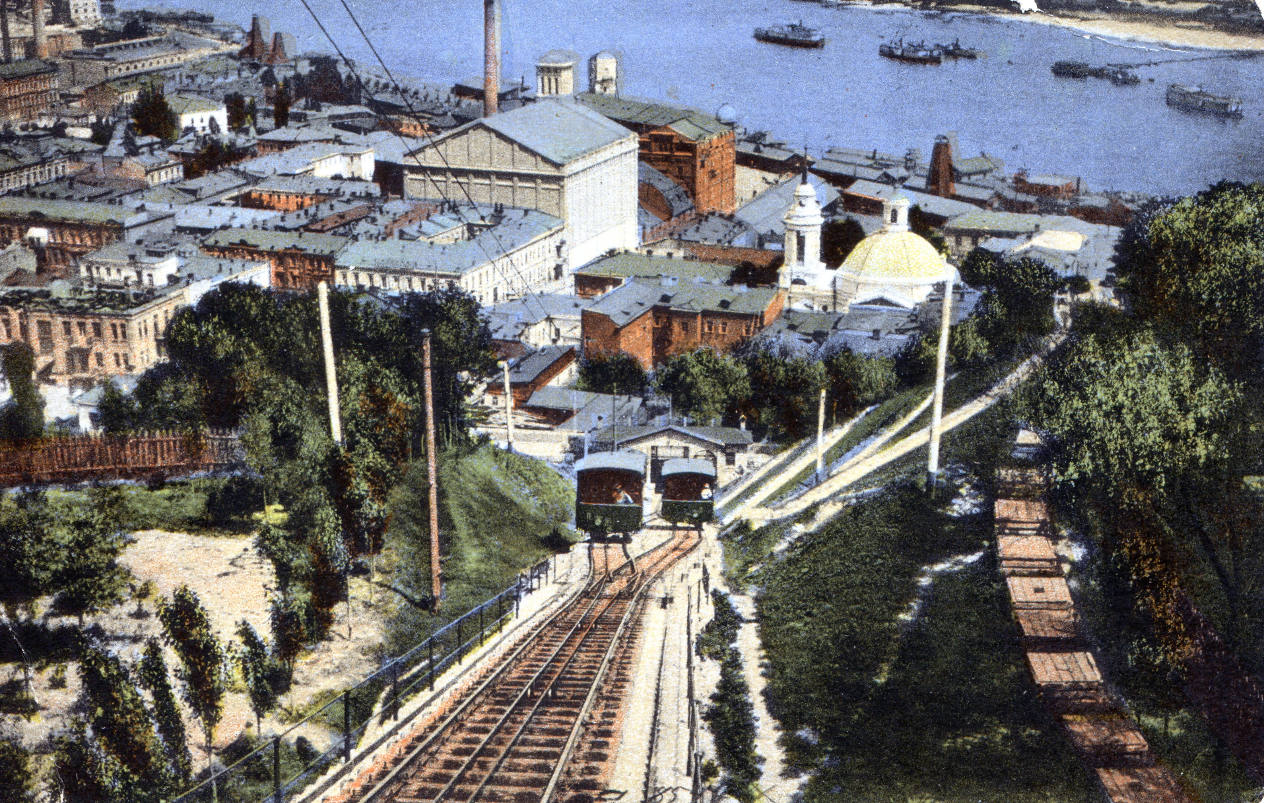
\includegraphics[width=\linewidth]{s-mihpod.jpg}
\end{center}

Старинная открытка с изображением оврага с фуникулером, вид с верхней площадки фуникулера. Собственно, Увоз Боричев.

\vspace*{\fill}

\newpage

\vspace*{\fill}

\begin{center}
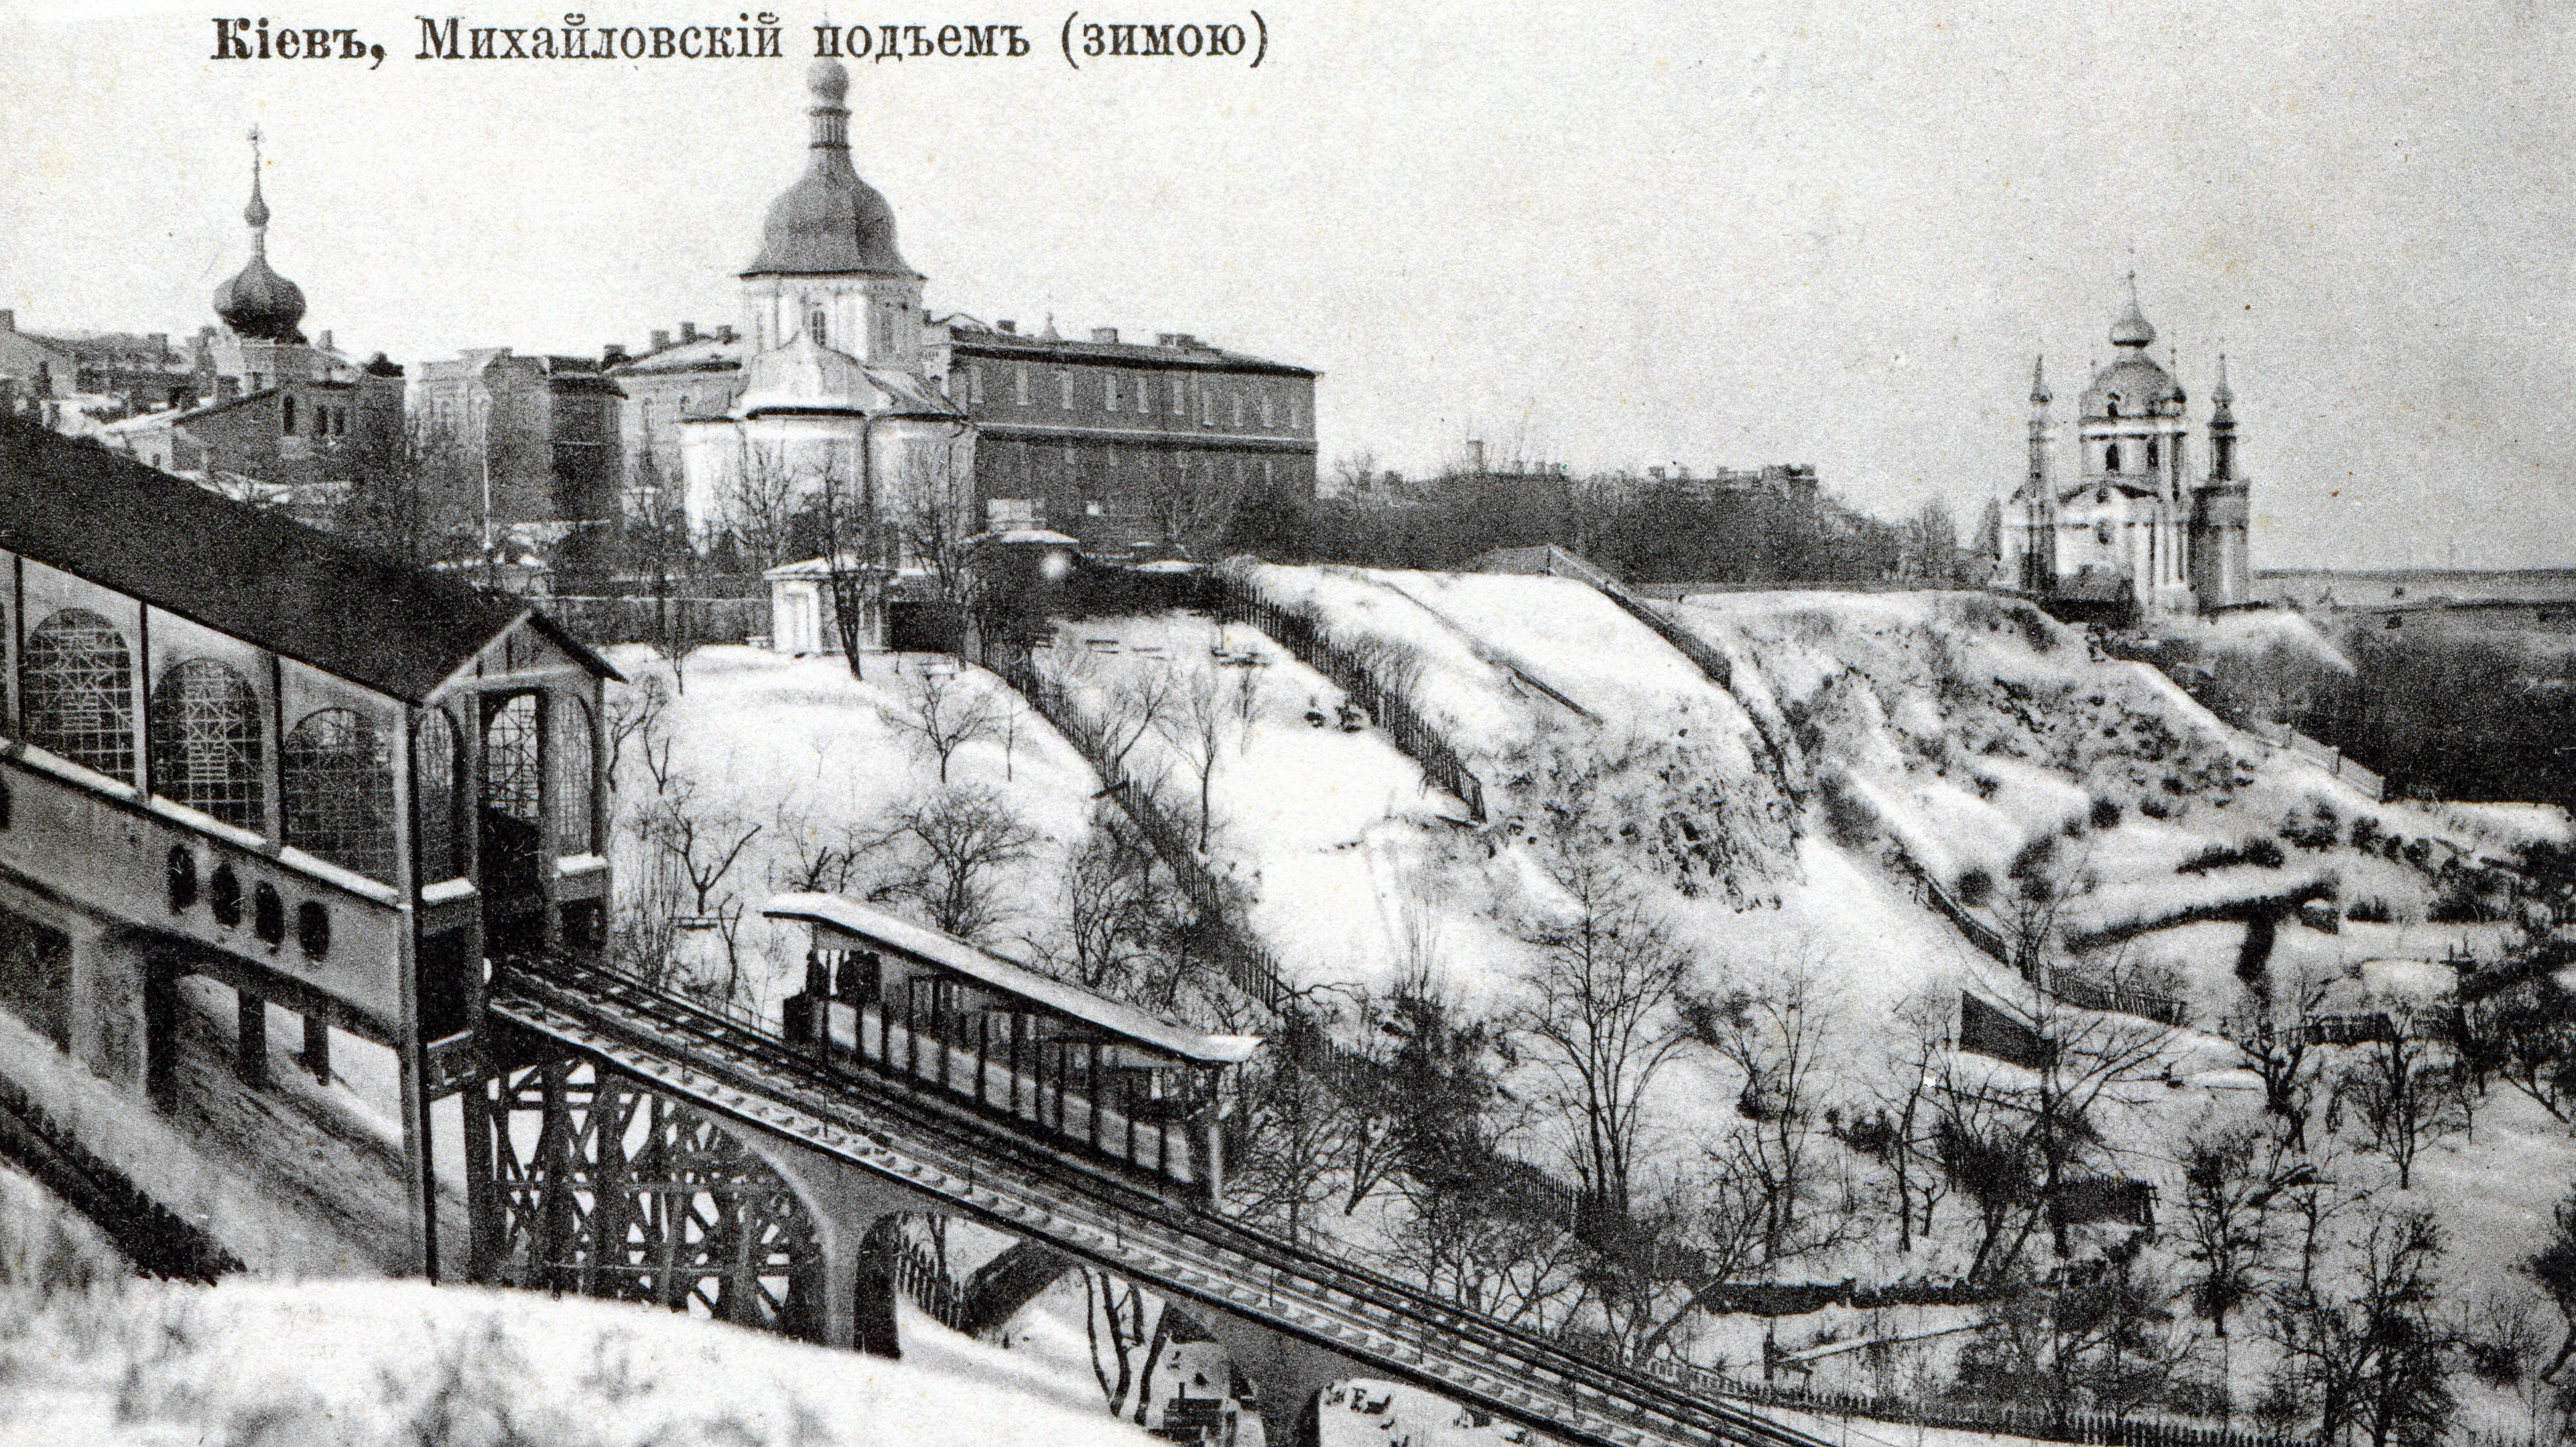
\includegraphics[width=\linewidth]{kuch01.jpg}
\end{center}

Место сада Кучинского на дореволюционной открытке, когда уже само название сада стёрлось из памяти и склоны эти называли Андреевской горой.

На переднем плане – фуникулер, тогда его называли «Михайловский подъем». Овраг над которым едет вагончик и есть Боричев.

За фуникулером – большая Трехсвятительская церковь, возможно на месте давней Васильевской, заложенной Владимиром.

Позади церкви видим здание Женских курсов, а справа в кадре – Андреевская церковь. И вот пространство на уступе между нею и фуникулером, эти склоны, по сути и есть сад Кучинского.

\vspace*{\fill}

\newpage

\vspace*{\fill}

\begin{center}
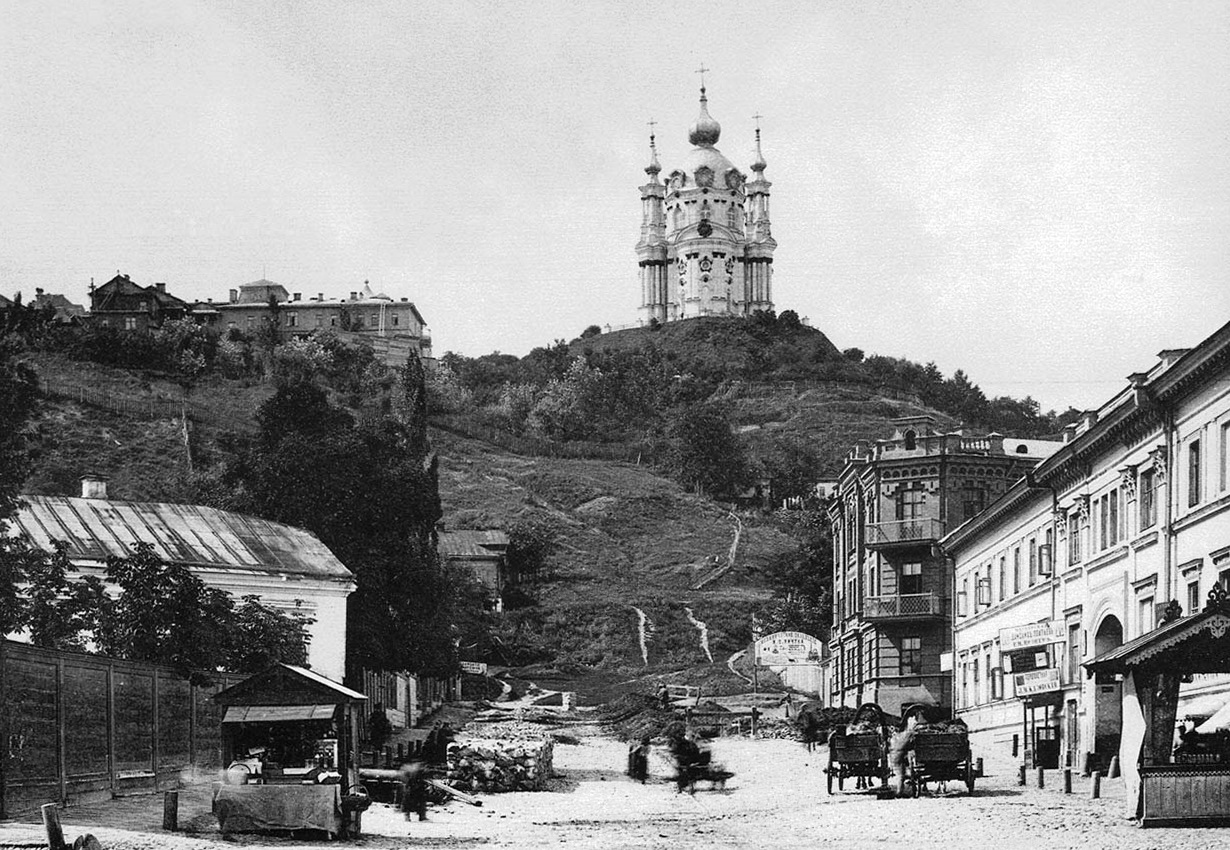
\includegraphics[width=\linewidth]{kuch02.jpg}
\end{center}

Вид с другого ракурса, на Андреевскую церковь, с улицы Андреевской, что на Подоле. Налево видим бывшее место сада Кучинского.

\vspace*{\fill}

\newpage

\vspace*{\fill}


\begin{center}
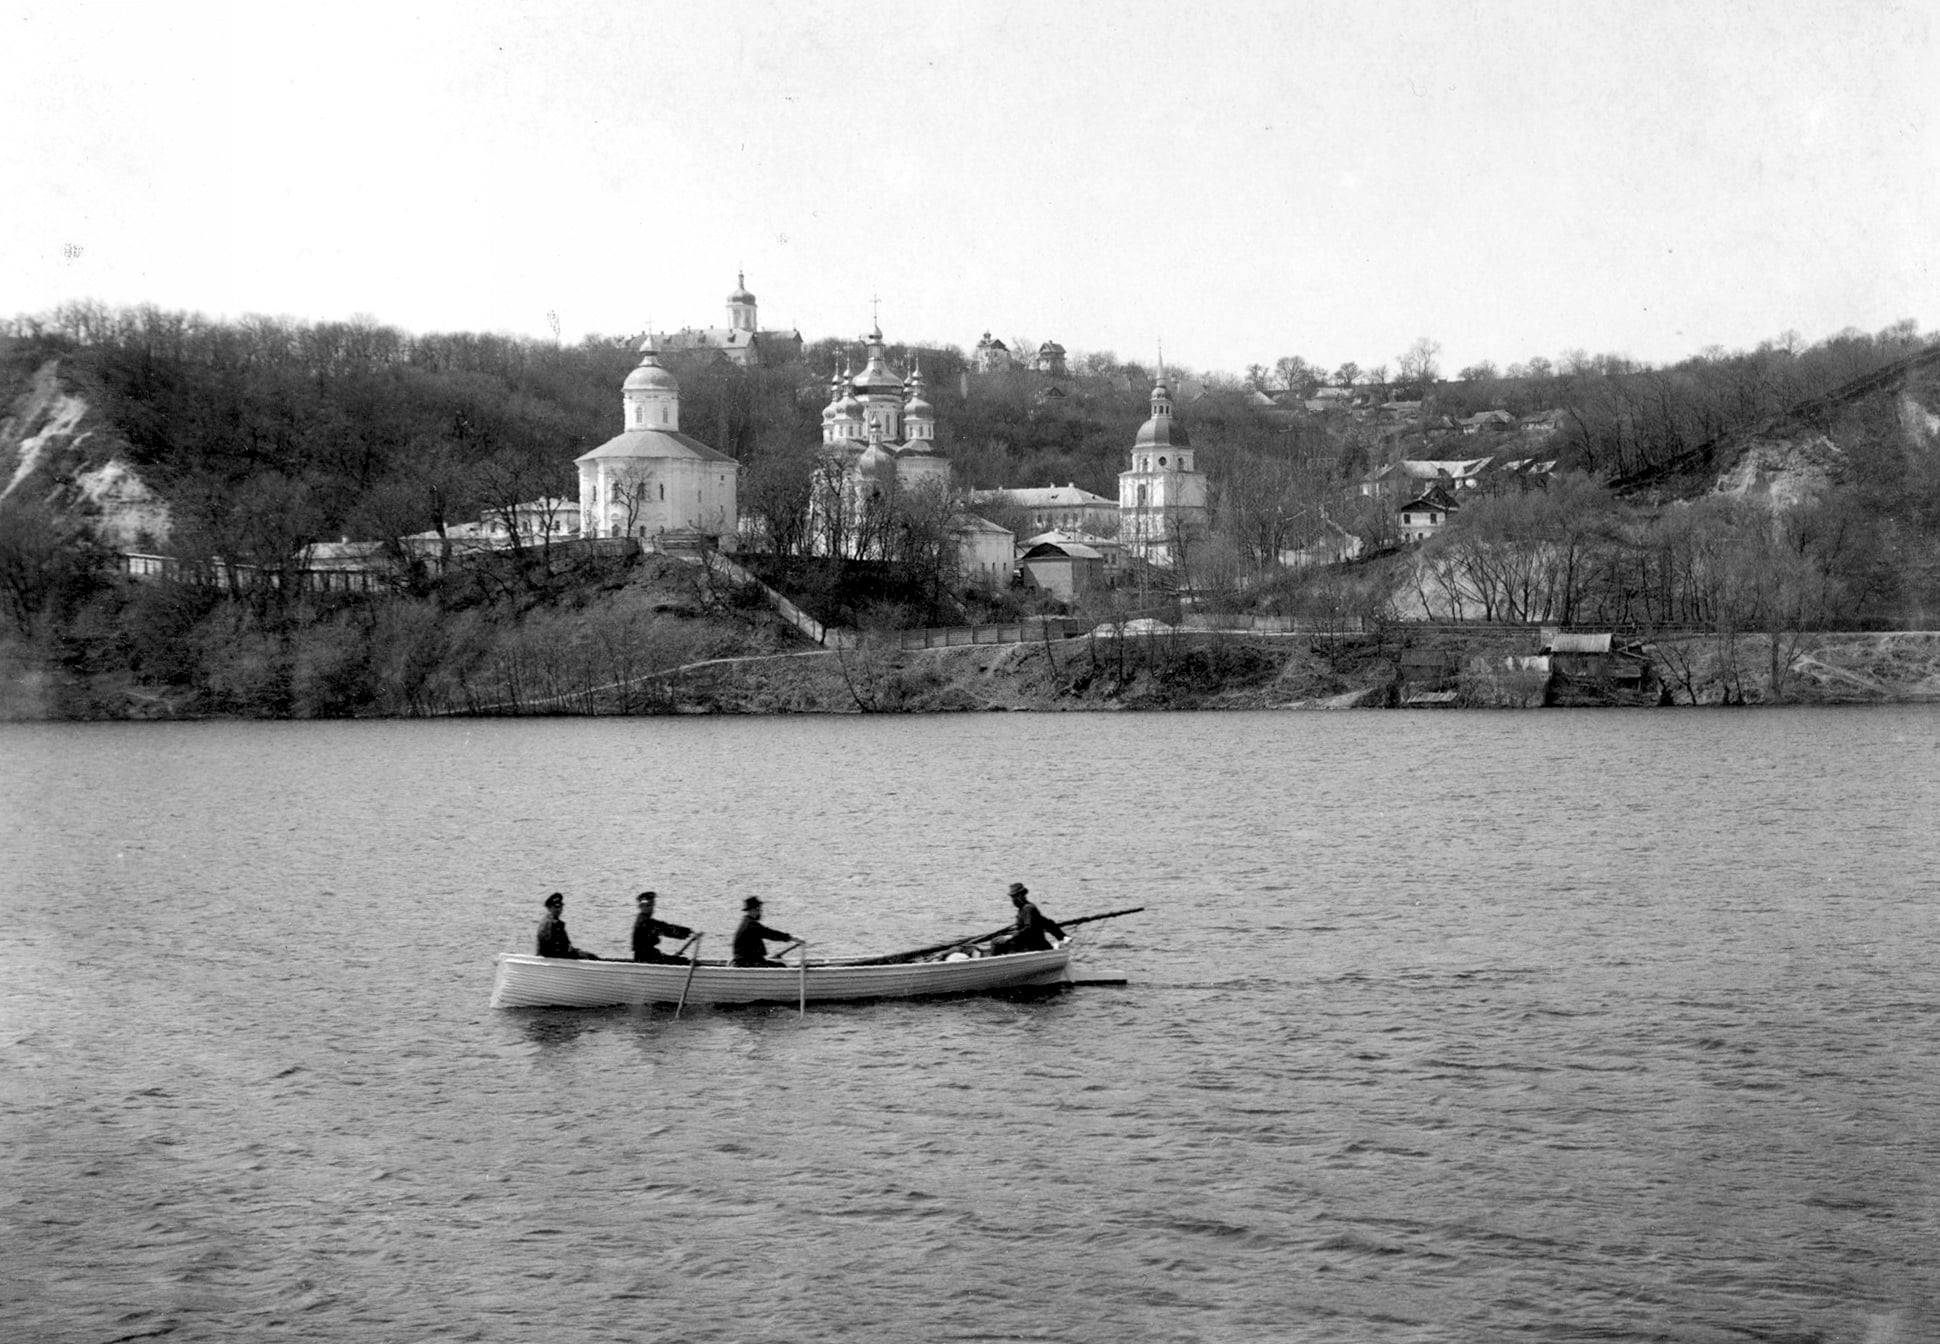
\includegraphics[width=\linewidth]{vyd01.jpg}
\end{center}

Вид на урочище Выдубичи и монастырь. Слева направо – храм чуда св. Михаила в Хонех, Георгиевский собор, Колокольня с церковью пророка Даниила. На горе наверху строения Ионинского Свято-Троицкого монастыря.

\vspace*{\fill}


\newpage

%\backmatter

%\appendix
%\addappheadtotoc


%\input{appendix/dict.tex}

\begin{thebibliography}{999}
\bibitem{zeleninrusalki}
\emph{Избранные труды. Очерки русской мифологии: Умершие неестественною смертью и русалки}. Зеленин Д. К. Индрик, Москва, 1995.

\bibitem{kak}
\emph{Как Владимир идолов низвергал}. Петр Семилетов, DOI 10.5281/zenodo.14212537

\bibitem{volos}
\emph{Скотий бог Волос}. Петр Семилетов, DOI 10.5281/zenodo.14563494
\end{thebibliography}


\end{document} 